\section{Auswertung}
\label{sec:Auswertung}
Tabelle \ref{tab:ein_eckig} zeigt die Messwerte der Auslenkung durch Kraft für einen eckigen Stab und \ref{tab:ein_rund} die Messwerte für einen runden Stab.
Beide Stäbe sind hierbei einseitig eingespannt worden.
In der Spalte $D_\text{A}(x)$ sind jeweils die absoluten Auslenkungen der Stäbe zu finden.
Diese wurde durch
\begin{equation}
    D_\text{A}(x) = D(x) - D_0(x)
    \label{eqn:Da}
\end{equation}
berechnet.
$D(x)$ steht hierbei für die Auslenkung an der Stelle $x$, während auf den Stab eine Kraft wirkt.
Die Spalte $D_0(x)$ zeigt die Auslenkung an der Stelle $x$, die der Stab hat bevor auf diesen eine Kraft wirkt.
$D_0(x)$ ist nicht an jedem Ort gleich, da die Stäbe nicht perfekt gerade sind.
Da die Stäbe außerdem nicht an jedem Punkt den selben Durchmesser haben, wurde dieser an zehn Stellen gemessen und die Messwerte gemittelt.
Der Mittelwert wurde für alle Berechnungen genutzt, bei denen dieser benötigt wird.
\begin{table}
\centering
\caption{Messwerte der Biegung für einseitige Einspannung.}
\subcaption{Messwerte für den eckigen Stab.}
\begin{tabular}[t]{cccc}
    \toprule
    $x\,/\,\si{\milli\meter}$ & $D_0(x) \,/\, \si{\milli\meter}$ & $D(x) \,/\, \si{\milli\meter}$ & $D_\text{A}(x) \,/\, \si{\milli\meter}$\\
    \midrule
    48.00 & 1.91 & 5.91 & 4.00 \\
    45.00 & 1.92 & 5.58 & 3.66 \\
    42.00 & 1.94 & 5.25 & 3.31 \\
    39.00 & 1.99 & 4.93 & 2.94 \\
    36.00 & 2.00 & 4.55 & 2.55 \\
    33.00 & 1.98 & 4.24 & 2.26 \\
    30.00 & 1.94 & 3.88 & 1.94 \\
    27.00 & 1.91 & 3.52 & 1.61 \\
    24.00 & 1.87 & 3.20 & 1.33 \\
    21.00 & 1.86 & 2.91 & 1.05 \\
    18.00 & 1.92 & 2.72 & 0.80 \\
    15.00 & 1.89 & 2.48 & 0.59 \\
    12.00 & 1.95 & 2.35 & 0.40 \\
    9.00 & 2.00 & 2.25 & 0.25 \\
    6.00 & 2.05 & 2.18 & 0.13 \\
    \bottomrule
    \label{tab:ein_eckig}
\end{tabular}
\subcaption{Messwerte für den runden Stab.}
\begin{tabular}[t]{cccc}
    \toprule
    $x\,/\,\si{\milli\meter}$ & $D_0(x) \,/\, \si{\milli\meter}$ & $D(x) \,/\, \si{\milli\meter}$ & $D_\text{A}(x) \,/\, \si{\milli\meter}$\\
    \midrule
    48.00 & 4.41 & 7.83 & 3.42 \\
    45.00 & 4.41 & 7.63 & 3.22 \\
    42.00 & 4.07 & 6.90 & 2.83 \\
    39.00 & 3.80 & 6.28 & 2.48 \\
    36.00 & 3.55 & 5.67 & 2.12 \\
    33.00 & 3.38 & 5.12 & 1.74 \\
    30.00 & 3.14 & 4.37 & 1.23 \\
    27.00 & 2.94 & 3.90 & 0.96 \\
    24.00 & 2.76 & 3.50 & 0.74 \\
    21.00 & 2.58 & 3.14 & 0.56 \\
    18.00 & 2.49 & 2.84 & 0.35 \\
    15.00 & 2.34 & 2.51 & 0.17 \\
    12.00 & 2.24 & 2.29 & 0.05 \\
    9.00 & 2.16 & 2.10 & -0.06 \\
    6.00 & 2.13 & 1.99 & -0.14 \\
    \bottomrule
    \label{tab:ein_rund}
\end{tabular}
\label{tab:einseitig_komplett}
\end{table}

In den Tabellen \ref{tab:beid_eckig} und \ref{tab:beid_rund} sind die Messwerte der beidseitig eingespannten Stäbe zu finden.
Dabei wurde $D_\text{A}(x)$ wie in \eqref{eqn:Da} berechnet.

\begin{table}
\centering
\caption{Messwerte der Biegung für beidseitige Einspannung.}
\subcaption{Messwerte für den eckigen Stab.}
\begin{tabular}[t]{cccc}
    \toprule
    $x\,/\,\si{\milli\meter}$ & $D_0(x) \,/\, \si{\milli\meter}$ & $D(x) \,/\, \si{\milli\meter}$ & $D_\text{A}(x) \,/\, \si{\milli\meter}$\\
    \midrule
    52.00 & 2.23 & 2.42 & 0.19 \\
    49.00 & 2.26 & 2.68 & 0.42 \\
    46.00 & 2.25 & 2.84 & 0.59 \\
    43.00 & 2.30 & 3.00 & 0.70 \\
    40.00 & 2.33 & 3.16 & 0.83 \\
    37.00 & 2.39 & 3.00 & 0.61 \\
    34.00 & 2.50 & 3.30 & 0.80 \\
    31.00 & 2.55 & 3.34 & 0.79 \\
    24.00 & 2.66 & 3.61 & 0.95 \\
    21.00 & 2.74 & 3.75 & 1.01 \\
    18.00 & 2.80 & 3.88 & 1.08 \\
    15.00 & 2.65 & 3.62 & 0.97 \\
    12.00 & 2.71 & 3.62 & 0.91 \\
    9.00 & 2.75 & 3.31 & 0.56 \\
    6.00 & 2.21 & 2.60 & 0.39 \\
    \bottomrule
    
    \label{tab:beid_eckig}
\end{tabular}
\subcaption{Messwerte für den runden Stab.}
\begin{tabular}[t]{cccc}
    \toprule
    $x\,/\,\si{\milli\meter}$ & $D_0(x) \,/\, \si{\milli\meter}$ & $D(x) \,/\, \si{\milli\meter}$ & $D_\text{A}(x) \,/\, \si{\milli\meter}$\\
    \midrule
    
    54.00 & 2.30 & 2.44 & 0.14 \\
    51.00 & 2.42 & 2.94 & 0.52 \\
    48.00 & 2.55 & 3.41 & 0.86 \\
    45.00 & 2.64 & 3.82 & 1.18 \\
    42.00 & 2.74 & 4.23 & 1.49 \\
    39.00 & 2.84 & 4.55 & 1.71 \\
    36.00 & 2.94 & 4.84 & 1.90 \\
    33.00 & 3.07 & 5.05 & 1.98 \\
    30.00 & 3.17 & 5.17 & 2.00 \\
    24.00 & 3.31 & 5.37 & 2.06 \\
    21.00 & 3.41 & 5.26 & 1.85 \\
    18.00 & 3.53 & 5.12 & 1.59 \\
    15.00 & 3.33 & 4.70 & 1.37 \\
    12.00 & 3.28 & 4.41 & 1.13 \\
    9.00 & 3.16 & 4.08 & 0.92 \\

    \bottomrule
    
    \label{tab:beid_rund}
\end{tabular}
\label{tab:beidseitig}
\end{table}


Zur Auslenkung der veschiedenen Stäbe wurden unterschiedliche Massen genutzt, diese sind in \ref{tab:massen} zu finden.
Zu beachten ist dabei, dass der eckige Stab sowohl für die beidseitige als auch für die einseitige Einspannung genutzt wurde, deshalb ist dieser zweimal in der Tabelle \ref{tab:massen} zu finden.
\begin{table}
\centering
\caption{Die Massen die für die Auslenkung der Stäbe genutzt wurden.}
\begin{tabular}{cccc}
    \toprule
   Stab & Auslenkungen & Masse $\:/\:\si{\kilo\gram}$ & Ort der Masse $\:/\:\si{\centi\meter}$ \\
    \midrule
    eckig 1  & \ref{tab:ein_rund} & 500.2 & 49 \\
    rund  1  & \ref{tab:ein_eckig} & 1711.6 & 49 \\
    eckig 1  & \ref{tab:beid_rund} & 2880.2 & 27.5 \\
    rund  2  & \ref{tab:beid_eckig} & 2880.2 & 27.5 \\
    \bottomrule
\end{tabular}
\label{tab:massen}
\end{table}


\FloatBarrier
\subsection{Der Elastizitätsmodul des eckigen Stabes}
Der eckige Stab dessen Auslenkungen in \ref{tab:ein_eckig} aufgetragen sind, hat die Eigenschaften die in Tabelle \ref{tab:eigen_eckig} dargestellt wurden.
\begin{table}
\centering
\caption{Werte für den eckigen Stab.}
\begin{tabular}{cc}
\midrule
    \text{Länge} L & \SI{59.1}{\centi\meter} \\
    \text{Seite} b & \SI{10.120(29)}{\milli\meter} \\
    \text{Seite} a & \SI{10.270(57)}{\milli\meter} \\
    \text{Masse} m & \SI{455.1}{\gram} \\
\bottomrule
\end{tabular}
\label{tab:eigen_eckig}
\end{table}
Damit hat dieser eine Dichte von $\SI{8.94(6)}{\gram\per\cubic\centi\meter}$.

Die durch die einseitige Biegung des Stabes aufgenommenen Werte sind in Abbildung \ref{fig:ein_eckig} in einem Plot dargestellt.
Dieser wurde mit den python Plugin \cite{matplotlib} erstellt.
Die Ausgleichsgerade folgt dabei der Funktion
\begin{equation}
    D(x) = F/(2\cdot E \cdot I) \cdot \left ( Lx^2 - \frac{x^3}{3} \right ).
    \label{eqn:ausgleich_ein}
\end{equation}
Wobei $I = \SI{9.14(16)e-10}{\meter^4}$ das Flächenträgheitsmoment darstellt.
Nach der Ausgleichsrechung ist der Wert für den Elastizitätsmodul $E = \SI{149.931(591)}{\giga\pascal}$.


\begin{figure}
\centering
\caption{Aufgetragene Messwerte für den eckigen Stab, bei einseitiger Einspannung.}
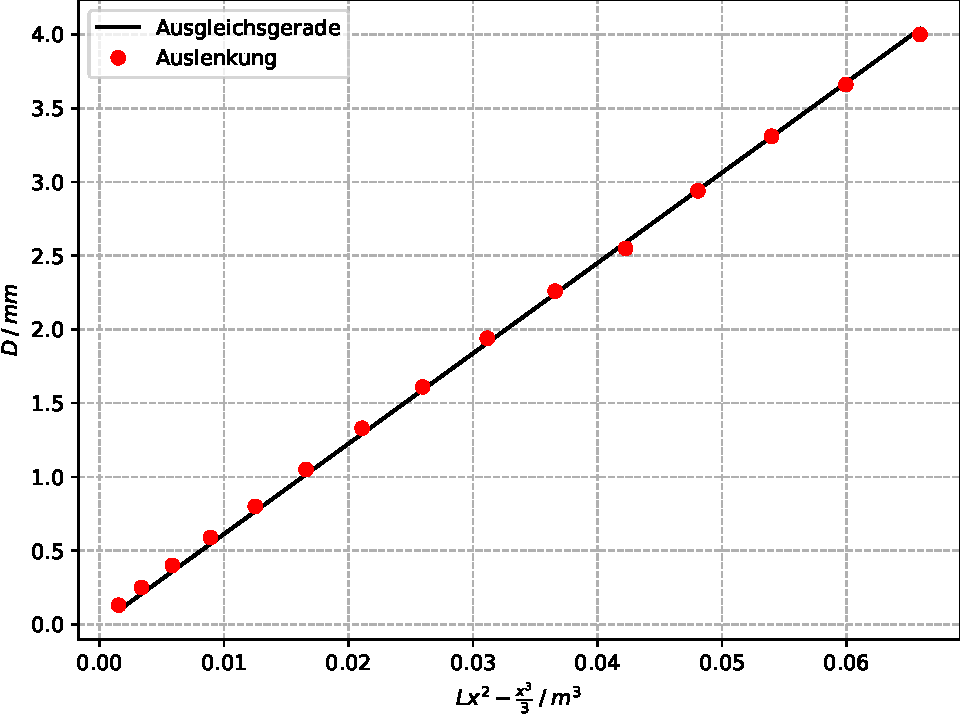
\includegraphics[width=\textwidth]{content/data/plot_einseitig_eckig.pdf}
\label{fig:ein_eckig}
\end{figure}

\begin{figure}
    \centering
    \caption{Beidseitige Einspannung des eckigen Stabes.}
    \begin{subfigure}{0.5\textwidth} 
       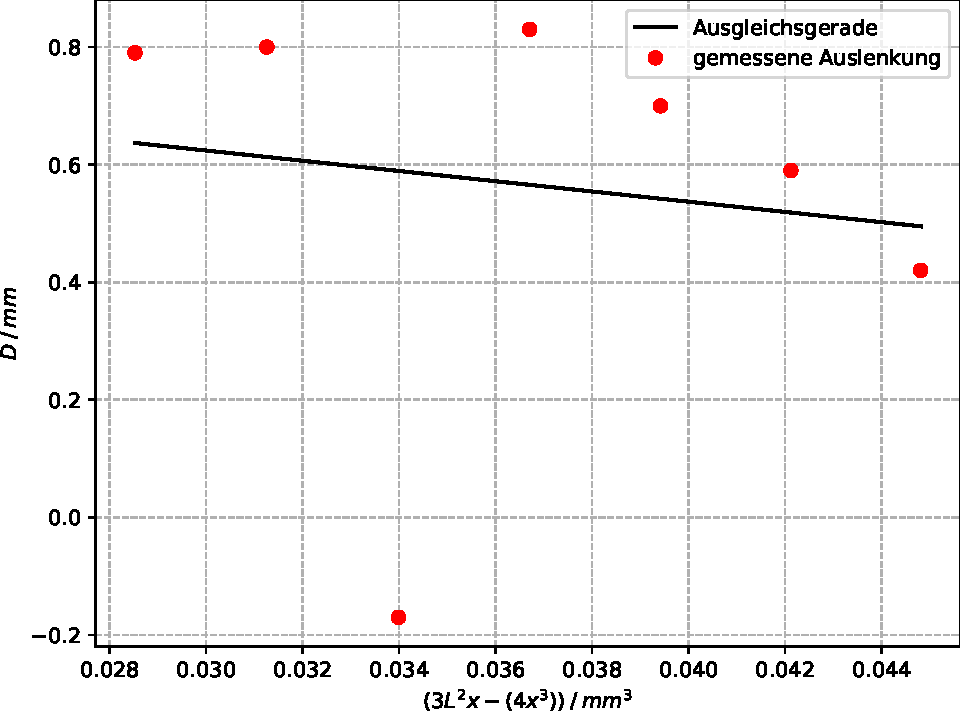
\includegraphics[scale=0.5]{content/data/plot_beidseitig_eckig_links.pdf}
       \caption{Die Auslenkung des Stabes links vom Gewicht.}
       \label{fig:beid_links_eckig}
    \end{subfigure}

    \begin{subfigure}{0.5\textwidth}
        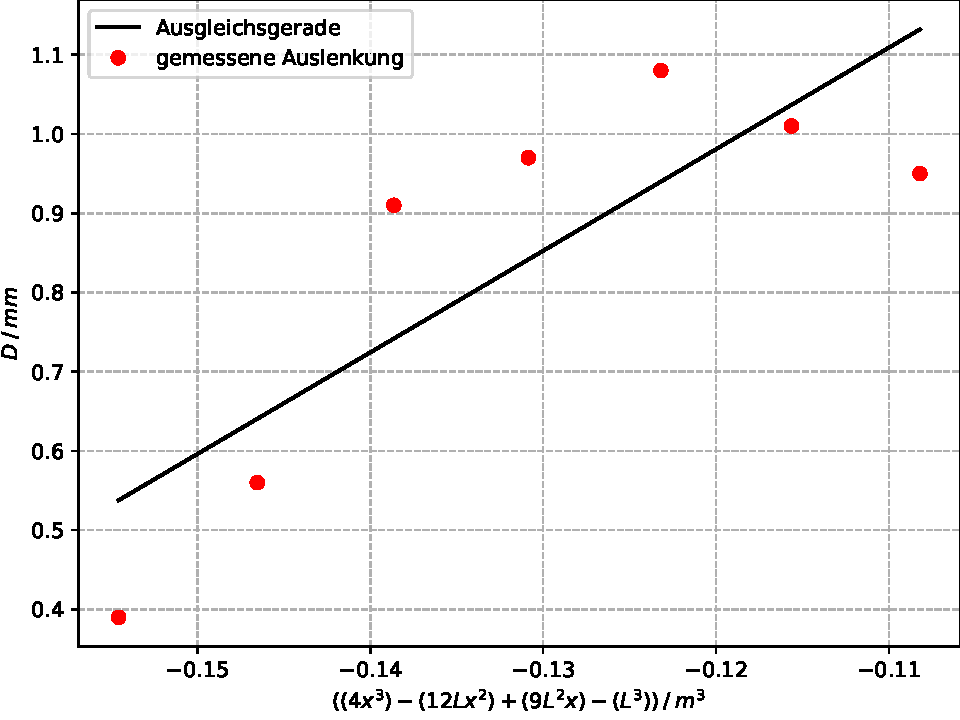
\includegraphics[scale=0.5]{content/data/plot_beidseitig_eckig_rechts.pdf}
        \caption{Die Auslenkung des Stabes rechts vom Gewicht.}
        \label{fig:beid_rechts_eckig}
    \end{subfigure}
    \label{fig:beid_eckig}
\end{figure}

Der selbe Stab wurde ebenfalls beidseitig eingespannt und in der Mitte belastet.
Die aufgenommen Messwerte sind in Tabelle \ref{tab:beid_eckig} zu finden und wurden in der Abbildungen \ref{fig:beid_eckig} grafisch dargestellt.
Die Ausgleichsgerade folgen der Funktion 
\begin{equation}
    ax+b.
    \label{eqn:ausgleich_beid}
\end{equation}
Durch die Ausgleichsrechung wurde für die Funktion in Abbildung \ref{fig:beid_links_eckig} der Wert $a = \SI{-0.009(27)}{}$ und $b = \SI{8.85(993)e-4}{}$ bestimmt.
Durch das selbe Schema wurden die Werte $a= \SI{0.013(4)}{}$ und $b=\SI{0.0025(5)}{}$ für die Funktion in Abbildung \ref{fig:beid_rechts_eckig} bestimmt.
Für den Elastizitätsmodul ergab die Ausgleichsrechung links vom Gewicht $E_\text{links} = \SI{0.6(23)e3}{\giga\pascal}$ und rechts vom gewicht $E_\text{rechts}=\SI{96(18)e2}{\giga\pascal}$.
Im Mittel ergibt sich einen Wert von $E=\SI{0.3(11)e3}{\giga\pascal}$.

\FloatBarrier

\subsection{Der Elastizitätsmodul des ersten runden Stabes}
Es wurden zwei verschiedene runde Stäbe genutzt, der erste wurde einseitig eingespannt, der zweite beidseitig.
Der Fall des ersten Stabes wird in diesem Abschnitt behandelt.
Der Stab hat die Eigenschaften die in Tabelle \ref{tab:eigen_rund1} dargestellt sind.
Die gemessenen Auslenkung sind in Tabelle \ref{tab:ein_rund} zu finden.

\begin{table}
\centering
\caption{Eigenschaften des runden  Stabes, der einseitig eingespannt wurde.}
\begin{tabular}{cc}
    \midrule
    \text{Länge} L & \SI{55}{\centi\meter} \\
    \text{Durchmesser} d & \SI{9.959(16)}{\milli\meter} \\
    \text{Masse} m & \SI{360.4}{\gram} \\
    \bottomrule
\end{tabular}
\label{tab:eigen_rund1}
\end{table}
Damit hat der runde Stab eine Dichte von $\SI{8.410(28)}{\gram\per\cubic\centi\meter}$.
Die gemessenen Auslenkung wurden in der Abbildung \ref{fig:ein_rund} mit dem python Plugin \cite{matplotlib} grafisch dargestellt.
Die Ausgleichsgerade folgt dabei der Funktion \eqref{eqn:ausgleich_ein}.
Dabei hat das Flächenträgheitsmoment einen Wert von $I = \SI{4.831(32)e-10}{\meter^4}$ hat.
Die Ausgleichsrechung ergibt für den Elastizitätsmodul einen Wert von $E = \SI{121.796(4012)}{\giga\pascal}$.


\begin{figure}
    \centering
    \caption{Plot zur Biegung bei einseitiger Einspannung des runden Stabes.}
    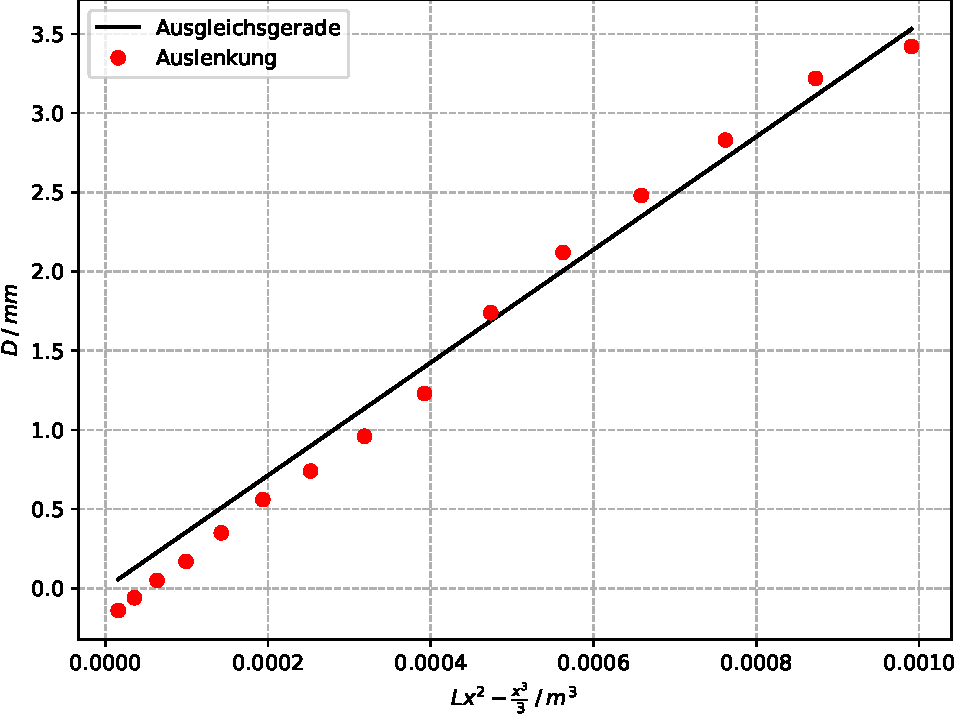
\includegraphics[scale=0.7]{content/data/plot_einseitig_rund.pdf}
    \label{fig:ein_rund}
\end{figure}

\FloatBarrier
\subsection{Der Elastizitätsmodul des zweiten runden Stabes}
Der zweite Runde Stab wurde beidseitig eingespannt.
Die Auslenkungen dieses Stabes sind in Tabelle \ref{tab:beid_rund} zu finden.
Die Eigenschaften des Stabes sind in Tabelle \ref{tab:eigen_rund2} zu finden.

\begin{table}
\centering
\caption{Die Eigenschaften des runden Stabes, der beidseitig eingespannt wurde.}
\begin{tabular}{cc}
    \midrule
    \text{Länge} L & \SI{60}{\centi\meter} \\
    \text{Durchmesser} d & \SI{10.010(10)}{\milli\meter} \\
    \text{Masse} m & \SI{132.6}{\gram} \\
\bottomrule
\end{tabular}
\label{tab:eigen_rund2}
\end{table}

Der Stab hat nach den in Tabelle \ref{tab:eigen_rund2} aufgetragenen Eigenschaften also eine Dichte von $\SI{2.808(6)}{\gram\per\cubic\centi\meter}$.
Die Messwerte wurden für die beiden Plots in Abbildung \ref{fig:beid_rund} grafisch dargstellt.
Dafür wurden zwei Ausgleichsgeraden erstellt die Gleichung \eqref{eqn:ausgleich_beid} folgen.
Für den Plot \ref{fig:beid_links_rund} wurde ein Wert von $a = \SI{-0.079(6)}{}$ und $b = \SI{4.916(291)e-3}{}$ genutzt.
Für den Plot \ref{fig:beid_rechts_rund} ergeben sich die Werte $a = \SI{0.019(2)}{}$ und $b = \SI{4.659(453)e-3}{}$.
Der Elastizitätsmodul lässt sich in diesem Fall durch die Ausgleichsrechung links vom Gewicht auf $E_\text{links} = \SI{89.3(22)}{\giga\pascal}$ setzten und rechts vom Gewicht auf $E_\text{rechts} = \SI{71(7)}{\giga\pascal}$ setzten. 
Im Mittel ergibt sich der Elastizitätsmodul $E = \SI{80(4)}{\giga\pascal}$.

\begin{figure}
    \centering
    \caption{Beidseitige Einspannung des runden Stabes.}
    \begin{subfigure}{0.4\textwidth} 
       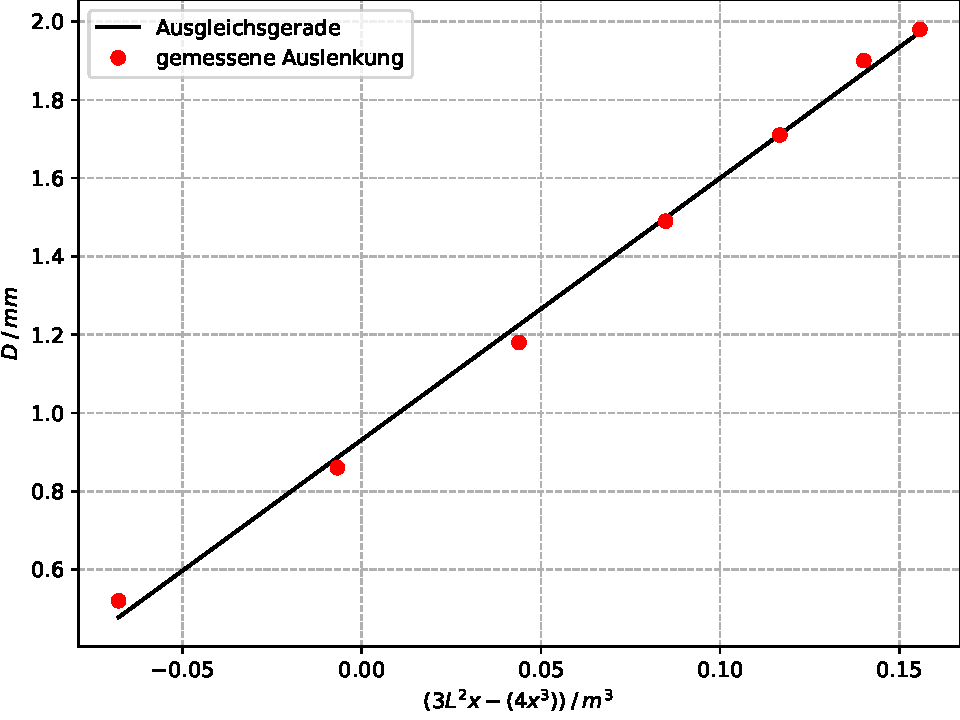
\includegraphics[scale=0.4]{content/data/plot_beidseitig_rund_links.pdf}
       \caption{Die Auslenkung des Stabes links vom Gewicht.}
       \label{fig:beid_links_rund}
    \end{subfigure}

    \begin{subfigure}{0.4\textwidth}
        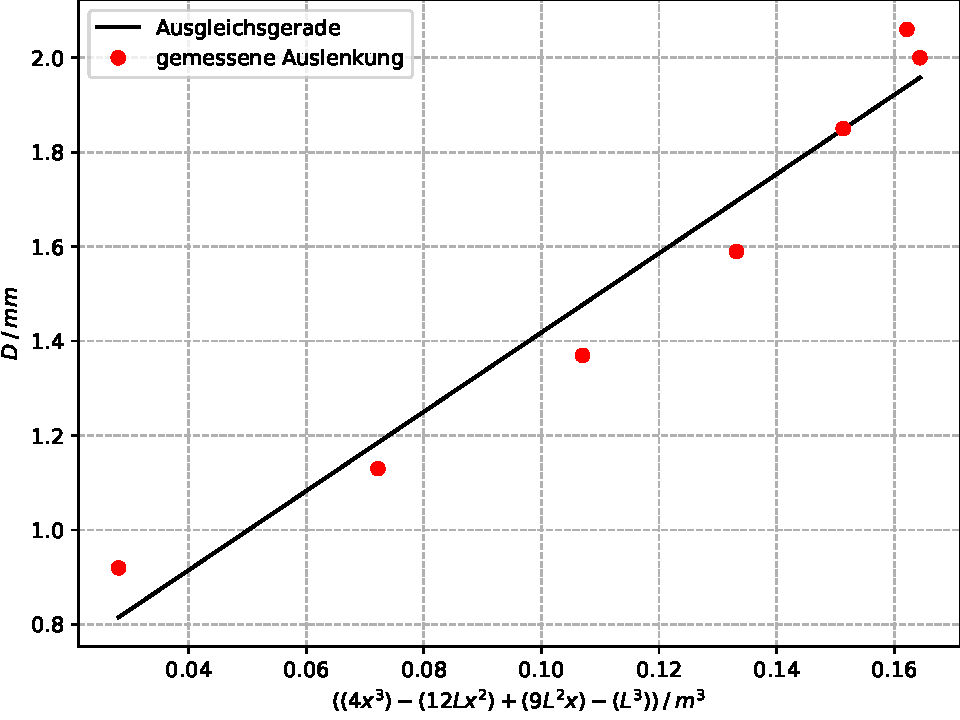
\includegraphics[scale=0.4]{content/data/plot_beidseitig_rund_rechts.pdf}
        \caption{Die Auslenkung des Stabes rechts vom Gewicht.}
        \label{fig:beid_rechts_rund}
    \end{subfigure}
    \label{fig:beid_rund}
\end{figure}

